\subsection{在 Gaudin 模型中的应用}\label{applic}

膜 $\Btriv$ 的自对偶性为文献~\cite{FFR,Frenkel} 的主要结果提供了一个规范理论解释：$\CP^1$ 上具有平凡单值性的 opers 对应于 Gaudin 模型对易哈密顿量的同时本征向量。我们考虑 $(\Bcc,\Btriv)$ 弦空间与 $(\Boper,\Btriv)$ 弦空间之间的对偶。以下讨论假定读者熟悉文献~\cite{GuWtwo} 的框架。

% [Tutor Note: 物理图像] 这里的逻辑链是：$(\Bcc,\Btriv)$ 弦的量子化给出 $\frak H=(\otimes_aR_a)^{SU(2)}$，而对易 Hamiltonians 作为 $(\Bcc,\Bcc)$ 弦作用于其上；$S$ 对偶把该问题换成 $(\Boper,\Btriv)$ 弦，后者在 $B$ 模型中就是两个经典膜的交点，于是“本征向量”变成“交点”，即具有平凡单值性的 opers。这就是 Gaudin 模型可积结构与 oper 几何之间的对偶的物理来源。

为构造 $(\Bcc,\Btriv)$ 弦空间，我们必须量子化模空间 $(\prod_{a=1}^d\CP^1_a)/SL(2,\C)$，其中 $\CP^1_a$ 是附着在 $z=z_a$ 处单值性缺陷上的一份 $\CP^1$。$\CP^1_a$ 的量子化给出 $SU(2)$ 的一个不可约表示 $R_a$，其自旋为 $j_a=k_a/2$；而 $(\prod_{a=1}^d\CP^1_a)/SL(2,\C)$ 的量子化给出一个量子 Hilbert 空间 $\frak H$，它是 $\otimes_a R_a$ 的 $SU(2)$ 不变部分，
\begin{equation}\label{ifo} \frak H=(\otimes_aR_a)^{SU(2)}. \end{equation}
Hitchin 可积系统的经典对易哈密顿量可以（在 $\omega_K$ 型 $A$ 模型中）解释为 $(\Bcc,\Bcc)$ 弦。因此它们作用于 $(\Bcc,\Btriv)$ 弦的空间 $\frak H$ 上。事实上，Hitchin 哈密顿量成为 Gaudin 模型的对易哈密顿量。为证明后一陈述，我们把 $R_a$ 上 $SU(2)$ 作用的生成元解释为来自 $\CP^1_a$ 上的一阶微分算子，于是 Gaudin 哈密顿量 (\ref{gaudham}) 成为二阶微分算子。这些算子的“符号”（即领头项的系数）是 Hitchin 纤维化底空间上的函数，而这些函数正是 Hitchin 哈密顿量。因此反过来读，Gaudin 哈密顿量表示 Hitchin 哈密顿量的一个量子化（而且鉴于 Hitchin 哈密顿量彼此对易，这一量子化在相差添加 $c$-数的意义下是唯一的）。

% [Tutor Note: 易错点] “量子化 $\CP^1_a$ 得到自旋 $j_a=k_a/2$ 的表示”用的是几何量子化：$\CP^1$ 的辛形式取为曲率 $\propto$ 面积形式，其预量子化线丛的次数即 $2j_a$，故 $2j_a=k_a$。若把 $\CP^1_a$ 的辛形式归一化取反或取倍，$j_a$ 会差整数倍，进而使 $\frak H$ 与 Gaudin 模型的谱不匹配；此处必须以第~\ref{mondr}~节中 $\lambda_a=k_a/2$ 的定义为准。

为理解对易哈密顿量的本征向量与本征值，我们利用 $\omega_K$ 型 $A$ 模型中的 $(\Bcc,\Btriv)$ 弦与 $J$ 型 $B$ 模型中的 $(\Boper,\Btriv)$ 弦之间的等价性。后一类弦简单地对应于经典膜 $\Bcc$ 与 $\Boper$ 的交点。因此，具有平凡单值性的 opers 给出 Gaudin 模型的量子 Hilbert 空间 $\frak H$ 的一组基。在 $B$ 模型的描述中，对易哈密顿量简单地成为 opers 簇 $\V$（即膜 $\Boper$ 的支撑）上的函数。Hitchin 的经典哈密顿量是 $C$ 上二次微分空间（在单值性缺陷位置 $z_a$ 处具有指定类型的极点）上的全纯函数。$\V$ 的支撑是 $C$ 上的应力张量空间（在 $z_a$ 处具有指定极点）。应力张量空间与二次微分空间之差仅在于 $c$-数的共形反常。这与 Hitchin 哈密顿量量子化中的加性 $c$-数不确定性相匹配。对应于给定 oper 的量子化哈密顿量的本征值，简单地由与该 oper 相联系的应力张量给出。

最近文献~\cite{NStwo} 描述了一种 Gaudin 模型的“非紧”版本，其中有限维表示 $R_a$ 被无限维表示取代。对易哈密顿量的本征向量再次用 opers 表达，只是对其单值性有某些条件。自然可以猜测这一构造同样反映了某个自对偶膜的存在。确实有一个很好的候选者——一个自对偶膜，它通过把单值性缺陷的端点（如图~\ref{ends} 那样）换成这类缺陷的汇合点来构造，如图~\ref{junctions} 那样。这样的汇合点由如下方式定义：取一个环绕该汇合点的小二维球面 $S$，在其上求解 Hitchin 方程，并在 $S$ 与各单值性缺陷的交点处具有奇点（奇点类型依赖于参数 $\alpha_a,\beta_a,\gamma_a,\eta_a$）。



 \begin{figure}
 \begin{center}
     % >>> 原文图 28（原稿第 108 页）
  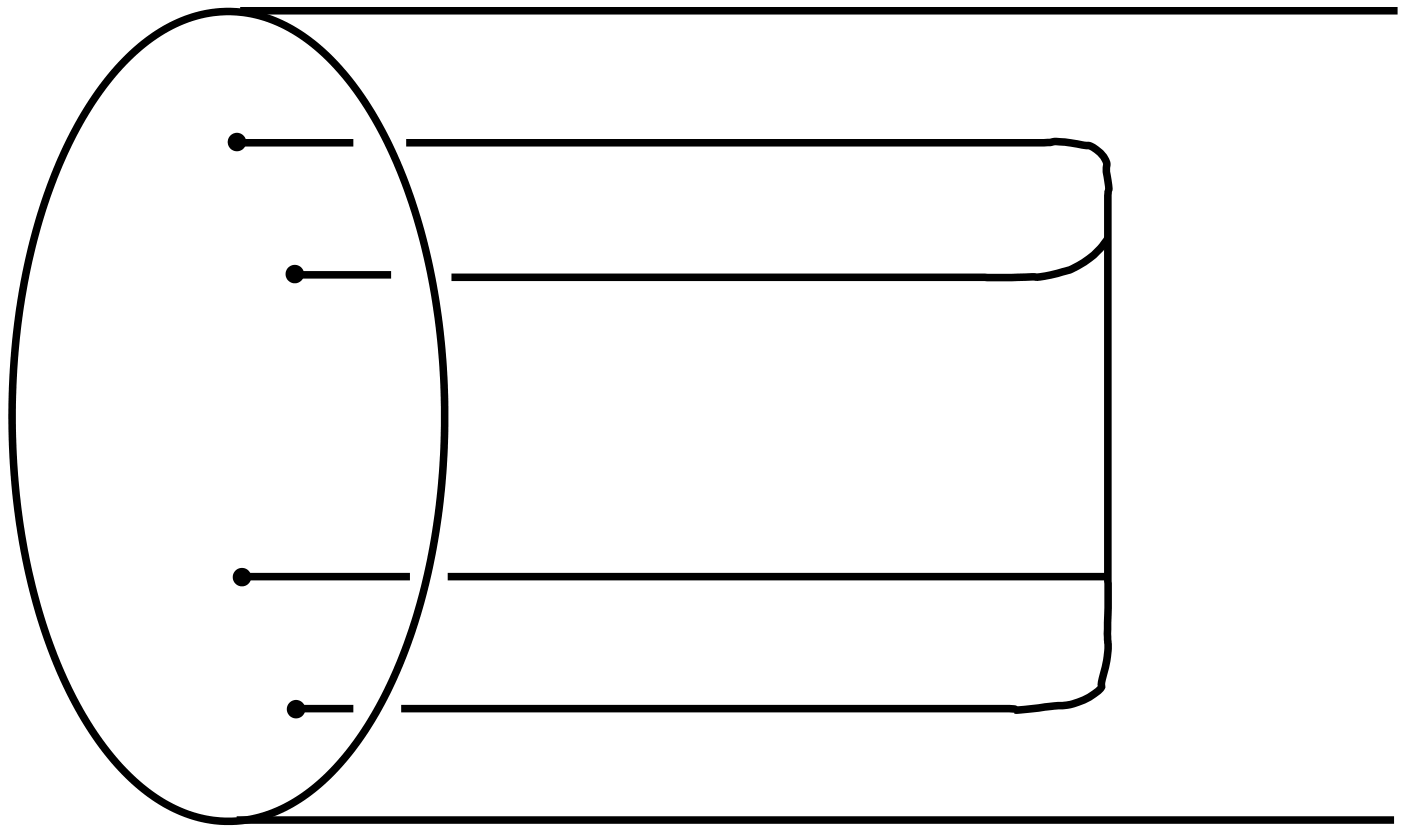
\includegraphics[width=3.5in]{figs/Fig28.png}
 \end{center}
\caption{\small  另一个自对偶膜可以通过把我们在图~\ref{ends} 中用到的单值性缺陷端点替换为单值性缺陷的汇合点来构造，如图所示。（原稿第 108 页）}
 \label{junctions}
\end{figure}

\vskip .5cm
{\bf 致谢} 我们感谢 D. Bar-Natan、L. Kauffman、S. Lewallen、P. Li、R. Mazzeo、G. Moore、R. Schoen、P. Seidel、L.-F. Tam 与 V. Toledano-Laredo 的讨论与评论。我们也感谢 M. Turansick 在作图方面的协助。

\appendix


\section{从六维得到的三维 BPS 方程}\label{fromsix}

\begin{keytakeaways}
\begin{itemize}\setlength{\itemsep}{2pt}
  \item \textbf{物理图像}：三维 BPS 方程可以由六维理论得到：要求场强（视为 $SO(6)$ 李代数元素）落在某个 $SU(3)$ 子代数内，再作维数约化；不同的 $SU(3)$ 嵌入在约化后给出不等价的三维方程族。
  \item \textbf{数学工具}：$SO(6)/U(3)\sim SU(4)/U(3)\sim \CP^3$ 参数化 $SU(3)\subset SO(6)$ 的嵌入，$SO(3)\times SO(3)$ 的转动作用（在六维旋量空间上即 $SO(4)\subset SU(4)$），Nahm 方程与 Nahm 极点。
  \item \textbf{主要结论}：方程族是实一维的，$(\ref{bpszeta})$ 是其一般代表；$\zeta$ 可通过 $SO(2)_\zeta$ 旋转改变（代价是 $\varphi$ 的 $(1+\zeta^2)$ 标度变换），旋转后的 Nahm 极点边界条件由此得到；$\zeta$ 的几何意义体现在 moment map 的系数矩阵 $\omega^{ab}$ 上，且 $\omega^{z \bar z}/\omega^{\bar z z}=\zeta^2$。
\end{itemize}
\end{keytakeaways}

我们在第~\ref{teqone}~节考虑的时间无关位形是三维 BPS 方程
\begin{equation} \label{sixbps}
[\D_i, \D_j]=0 \qquad  \sum_{i=1}^3[\D_i,\D_i{}^\dagger]
\end{equation}
的解，其中的三维联络与三个伴随标量场被一起打包进算子 $\D_i$：
\begin{align} \D_1 & = \frac{D}{Dx^2}+i\frac{D}{Dx^3}    \cr
                                   \D_2 & = [\phi_2-i\phi_3,\,\cdot\,] \cr
                             \D_3 & = \frac{D}{Dy}-i[\phi_1,\,\cdot\,]  \end{align}
或者用复记号写成
\begin{align}\label{oggi} \D_1 & =2\frac{D}{D\bar z} \cr
                                                              \D_2 & = 2[\varphi,\,\cdot\,]\cr
                                                               \D_3& = \frac{\D}{\D y}. \end{align}
该方程组可以推广为含一个实参数的三维 BPS 方程族，其形式与 \ref{sixbps} 相同，但算子 $\D_i$ 的选择不同：
\begin{align}\label{bpszeta}\D_1 & =2\frac{D}{D\bar z}  +2 \zeta [\bar \varphi,\,\cdot\,] \cr
                                                              \D_2 & = - 2 \zeta \frac{D}{D z} + 2[\varphi,\,\cdot\,]\cr
                                                               \D_3& = \frac{\D}{\D y}. \end{align}
这一推广曾在第~\ref{analog}~节研究过。



这一族三维方程可以从六维有效地导出。我们从坐标 $x^a,$ $x^{a+3}$（$a=1,2,3$）的 $\R^6$ 出发，然后对规范场施加约束：要求场强（视为 $SO(6)$ 李代数中的元素）落在某个指定的 $SU(3)$ 子群内。只要还在六维中，子群的选择就无关紧要；它只相当于选定 $\R^6$ 与 $\C^3$ 的一个等同方式。但若我们要求各场实际上只依赖于前三个坐标 $x^a$，并在 $x^{a+3}$ 的常数平移下不变，那么 $SU(3)$ 子群的选择就变得重要了。因此在约化到三维之后，可以得到一个依赖于参数的、彼此不等价的三维方程组族。



要说明该族（模去等价）是实一维的，一个简单办法如下。首先，$SU(3)$ 在 $SO(6)$ 中的嵌入选择由 $SO(6)/U(3)\sim SU(4)/U(3) \sim \CP^3$ 参数化，它等价于在正手征的六维旋量空间中选定一条复直线。约化到三维后，不等价的三维方程组由这样的选择模去空间转动与三个标量 $\phi_i$ 转动的 $SO(3) \times SO(3)$ 群参数化。虽然该群与 $\CP^3$ 一样是六维的，但它在 $\CP^3$ 上的作用并不自由；相反，$\CP^3$ 中的一般点保持 $SO(3)\times SO(3)$ 的一个 $SO(2)$ 子群。例如，由 $\zeta$ 参数化的所有三维方程在 $D/Dz$ 与 $\phi_z$ 同时作相位转动下不变。一般地，$SO(3) \times SO(3)$ 在六维旋量空间上的作用相当于 $SO(4) \subset SU(4)$。因此 $SU(4)$ 的一个复旋量是 $SO(4)$ 的一个复向量，其实部与虚部分别把 $SO(4)$ 破缺到 $SO(2)$。于是，作为六维方程的维数约化而得到的三维方程组族是实一维的，而 (\ref{bpszeta}) 是一般的代表。

这一图像的一个推论是，我们可以用 $SO(6)$ 转动来改变 $\zeta$。确实，通过作用一个我们记作 $SO(2)_\zeta$ 的群中的适当元素，就可以按需要改变 $\zeta$；该群把 $D/Dx^2$ 与 $[\phi_2,\,\cdot\,] $ 相互转动，也把 $D/Dx^3$ 与 $[\phi_3,\,\cdot\,]$ 相互转动。确切地说，作用在 $\zeta=0$ 处定义的 $\D_i$ 上的 $SO(2)_\zeta$ 转动将给出略微标度过的 $\D_i$，带一个前因子 $(1+\zeta^2)^{-1/2}$。该前因子可以通过对 $z$ 坐标作简单的标度变换而吸收掉。

现在我们讨论本文中十分重要的 Nahm 极点边界条件。若假定各场只依赖于 $y$，并进一步假定 $A_{\bar z}=0$（从而可以不顾 $\D_1$），则取 (\ref{oggi}) 中 $\D_i$ 的方程 (\ref{sixbps}) 约化为 Nahm 方程。Nahm 极点边界条件定义为要求 $y\to 0$ 时各场可以用 Nahm 方程的某个奇异解来近似。


对一般 $\zeta$ 的三维 BPS 方程也有类似的边界条件。确实，$SO(2)_\zeta$ 把只依赖于 $y$ 的 (\ref{sixbps}) 的解映为只依赖于 $y$ 的 (\ref{bpszeta}) 的解。更显式地，取 (\ref{bpszeta}) 中 $\D_i$ 的一般形式，我们可以寻找只依赖于 $y$、且使 $\D_1$ 约化为 $2\partial/\bar\partial\bar z$ 的解，即 $A_{\bar z} =- \zeta \bar \varphi$。于是 $\D_2 =  2(1 + \zeta^2) [\varphi,\,\cdot\,]$，从而我们可以把 Nahm 方程的解嵌入为一般三维 BPS 方程的解，代价是把复标量 $\varphi$ 标度 $1+ \zeta^2$ 倍。这就引出了我们在本文中发现有用的旋转后 Nahm 极点边界条件。

% [Tutor Note: 原文笔误] 此处原文作 “$\D_1$ reduces to $2\partial/\bar\partial\bar z$”，按上下文与 $\D_1=2D/D\bar z$（$D/D\bar z=\partial/\partial\bar z+[A_{\bar z},\,\cdot\,]$，当 $A_{\bar z}=-\zeta\bar\varphi$ 时其纯导数部分为 $2\partial/\partial\bar z$）判断，应为 $2\partial/\partial\bar z$。原式如此，未改。

当然，我们刚才描述的并非与一般三维 BPS 方程相容的唯一 Nahm 极点嵌入方式。例如，在 $\zeta \neq 0$ 时，我们本可以选择另一种嵌入，使 $\D_2$ 而非 $\D_1$ 是平凡的；那将引出我们或可称为反 opers 的对象——即平坦丛，其 oper 型约束加在反全纯结构而非全纯结构上。把我们所选的 Nahm 极点用 $SU(3)$ 中保持 $\D_3$ 的 $U(2)$ 子群作任意转动，都会产生一个可能的边界条件，但我们将一般坚持用“oper”型 Nahm 极点。

最后，我们对参数 $\zeta$ 的含义给出另一种解释。对有限非零的 $\zeta$，可以对 $\D_i$ 作标度变换，并将其解释为一般的复三维联络。在直角坐标中，可把联络的各分量记为 $\tilde \D_a$。复方程告诉我们该联络是平坦的。然后我们有一个 moment map 约束，它令对易子 $[\tilde \D_a, \tilde \D^\dagger_b]$ 的某个常系数线性组合为零。

从这一观点看，$\zeta$ 只出现在 moment map 方程的选取中。对易子的一般线性组合由系数构成的 $3 \times 3$ 矩阵 $\omega^{ab}$ 描述，
\begin{equation}\label{mct}  \sum_{a,b} \omega^{ab} [\tilde \D_a,\tilde \D_b{}^\dagger]=0.
\end{equation}
由式 (\ref{bpszeta}) 可得一个有用的关系：$\omega^{z \bar z}/\omega^{\bar z z}=\zeta^2$。若 $\zeta^2=1$，则 $\omega^{ab}$ 是对称的，但一般并非如此。

一般地，在线性坐标重定义下，可能的 $\omega^{ab}$ 构成一个一维参数空间。例如，若 $\omega^{ab}$ 的对称部分是正定的（对 (\ref{bpszeta}) 而言确实如此），我们可以把它化为单位矩阵 $\delta^{ab}$。此时反称部分 $B^{ab}$ 可以转动到只存在于 $z, \bar z$ 平面内，其大小由一个实参数控制，我们可以把这个参数等同于 $\zeta$。

\section{从四维与八维得到的三维 BPS 方程}\label{foureight}

\begin{keytakeaways}
\begin{itemize}\setlength{\itemsep}{2pt}
  \item \textbf{物理图像}：四维 BPS 方程 (\ref{bpseqns}) 可看作八维 Yang-Mills 中 BPS 方程的维数约化；把 $x^1$ 方向去掉并把 $A_1,\phi_y$ 取为 $\vec\phi$ 的线性组合，就得到三维 BPS 方程，其参数 $\zeta$ 由该组合决定。
  \item \textbf{数学工具}：八维 $\mathrm{Spin}(8)$ 手征旋量 $\epsilon$、条件 $F_{IJ}\Gamma^{IJ}\epsilon=0$、$\mathrm{Spin}(7)\subset SO(8)$ 与 $SO(6)\to SU(3)$ 的嵌入链、升降算符 $\gamma_{\underline a},\gamma_{\overline a}$ 与真空 $|\Omega\rangle,|\mho\rangle$、$\tau=\tan\alpha$。
  \item \textbf{主要结论}：四维方程 (\ref{dolk}) 由八维方程约化得到且 $\t=\tan\alpha$；只依赖于部分坐标的解保持额外超对称（$F_{I8}=0$ 给出 $SO(7)\to G_2$；再加上 $F_{I7}=0$ 给出 $SO(6)\to SU(3)$ 及三维 BPS 方程）；显式做法是绕 $(a,a+4)$ 平面作 $SO(2)$ 转动，$\zeta=\tan\theta_2$，且取 $\theta_1=-2\theta_2=-2\theta_3=-2\theta$ 时保持 $\t=1$、只形变 Nahm 极点边界条件。
\end{itemize}
\end{keytakeaways}

在本附录中，我们将讨论参数为 $\zeta$ 的三维 BPS 方程如何能从四维 BPS 方程 (\ref{bpseqns}) 的时间无关解得到。我们将推广如下陈述：三维中 $\zeta=0$ 的方程来自四维中 $\t=1$ 的方程，只要我们丢掉对某个坐标（比如 $x^1$）的依赖，并令 $A_1=\phi_y=0$。

首先我们将说明这并不是某个特定选择所特有的性质。我们可以从任意 $\t$ 出发，令 $\d/\d x^1=0$，并把 $A_1$ 与 $\phi_y$ 取为 $\phi$ 的其余三个分量的任意两个线性组合，则所得的三维方程将等价于上一附录中讨论的三维 BPS 方程，对 (\ref{bpszeta}) 中参数 $\zeta$ 的某个取值成立。

为此，把四维 BPS 方程改写为紧致形式（即八维 Yang-Mills 理论中 BPS 方程的维数约化）相当方便。描述所需八维方程的一个简洁方式是：取一个具有确定手征性的 $\mathrm{Spin}(8)$ 旋量 $\epsilon$，并要求
\begin{equation}
F_{IJ} \Gamma^{IJ} \epsilon =0.
\end{equation}
若把曲率 $F_{IJ}$ 理解为 $SO(8)$ 李代数中的元素，则这些方程把曲率限制在 $SO(8)$ 的 $\mathrm{Spin}(7)$ 子代数中。由于如下显然的关系，这些其实只是 7 个方程：
\begin{equation}
\epsilon^T F_{IJ} \Gamma^{IJ} \epsilon =0,
\end{equation}
因为 $\Gamma^{IJ}$ 是反称的。

约化到四维把 $SO(8)$ 破缺为一个我们记作 $SO(4)_s \times SO(4)_R$ 的子群，它分别作用在前四个与后四个坐标上。旋量 $\epsilon$ 分解为在 $SO(4)_s$ 与 $SO(4)_R$ 下均为左手征的一片 $\epsilon_L$，以及在 $SO(4)_s$ 与 $SO(4)_R$ 下均为右手征的一片 $\epsilon_R$。若 $\epsilon_L$ 与 $\epsilon_R$ 都非零，则它们选定一个对角地嵌在 $SO(4)_s \times SO(4)_R$ 中的扭化 $SO(4)'_s$，使得 $\epsilon_L$ 与 $\epsilon_R$ 都是 $SO(4)'_s$ 标量。于是那 $7$ 个方程在 $SO(4)'_s$ 下分解为三个自对偶二形式、三个反自对偶形式和一个标量方程。这正是 (\ref{bpseqns}) 中熟悉的形式。


\def\a{{\underline a}}
\def\aa{{\overline a}}
\def\b{{\underline b}}
\def\bb{{\overline b}}
我们把 $a'$ 作为 $a+4$ 的简写，并采用复记号，其中 $\a$ 是 $a+ia'$ 的简写，$\aa$ 是 $a-ia'$ 的简写。为把八维方程显式地化成 (\ref{bpseqns}) 的形式，把 $\Gamma$ 矩阵组合成升算符
\begin{equation}
\gamma_\a = \Gamma_a + i \Gamma_{a+4}
\end{equation}
与降算符
\begin{equation}
\gamma_{\aa} = \Gamma_a - i \Gamma_{a+4}
\end{equation}
是有用的，其中 $a=1,\dots,4$。我们把被降算符湮灭的态记作 $|\Omega\rangle$，把它的复共轭（即被升算符湮灭的态）记作 $|\mho\rangle$。由于在 $SO(4)'_s$ 下不变，$\epsilon$ 是 $|\Omega\rangle$ 与 $|\mho\rangle$ 的线性组合；由于是实的，它实际上是 $\epsilon =e^{-i \alpha} |\Omega \rangle+e^{i\alpha}|\mho\rangle$，其中 $\alpha$ 为某个实数。


于是，八维方程可以用曲率的 $(2,0)$、$(1,1)$ 与 $(0,2)$ 分量 $F_{\a\b}$、$F_{\a \bb}$ 与 $F_{\aa\bb}$ 写出：
\begin{align}
e^{-i \alpha}  F_{\a\b} + e^{i \alpha} \frac{1}{2} \epsilon_{ab}\,^{cd} 
F_{\overline c \overline d} &=0 \cr \sum_a F_{\a \aa}&=0.
\end{align} 
约化到四维时，第一个方程告诉我们 $ {\mathrm {Re}} \, (e^{-i \alpha} F_{\a \b}) $ 的自对偶部分为零，而 $ {\mathrm {Im}} \,( e^{-i \alpha} F_{\a\b}) $ 的反自对偶部分也为零。取 $\phi=\sum_a A_{a+4}\,\d x^a$，我们就还原出熟悉的四维方程
\begin{align} \label{dolk}(F-\phi\wedge \phi + \t \,\d_A\phi)^+&=0   \cr
                             (F-\phi\wedge\phi-\t^{-1}\d_A\phi  )^- &=0 \cr
                               \d_A\star\phi&=0,                     \end{align}                                                                    
其中 $\t = \tan \alpha$。

若从方程的八维形式出发，则显然有：不依赖于八个方向中某些方向的解保持额外的超对称。例如，任何满足 $F_{I8}=0$（对某个 $I$）的解也满足
\begin{equation}
F_{IJ} \Gamma^{IJ} \Gamma^8 \epsilon =0
\end{equation}
从而保持由 $SO(8)$ 的实反手征旋量 $\Gamma^8 \epsilon$ 所生成的那个超对称。那 7 个方程仍相互独立，并描述把 $SO(7)$ 约化到 $G_2$、同时保持一个七维旋量 $\epsilon_7$ 的情形。

满足 $F_{I8}=0$ 与 $F_{I7}=0$ 的解一般保持四个旋量：$\epsilon$、$\Gamma^7 \epsilon$、$\Gamma^8 \epsilon$、$\Gamma^{78} \epsilon$。此时那 7 个方程描述把 $SO(6)$ 约化到 $SU(3)$、并保持由六维复旋量 $\epsilon_6$ 及其复共轭所生成的超对称的情形。它们分解为 $3$ 个复方程与一个实 moment map 条件
\begin{equation}
[\D_i, \D_j]=0 \qquad \sum_i [\D_i, \D^\dagger_{\bar i}] =0,
\end{equation}
正如附录~\ref{fromsix} 所讨论的。

这正是我们在如下情形中所处的状况：在四维方程 (\ref{dolk}) 中，对任意 $\t$，我们令 $\d/\d x^1=0$，并把 $A_1$、$\phi_y$ 取为 $\phi$ 中其余三个标量场 $\vec \phi$ 的任意两个线性组合。任何这样的选择都会给出六维 BPS 方程的一个三维约化，从而按附录~\ref{fromsix} 的分析，将与某个 $\zeta$ 的标准三维 BPS 方程等价。
% [Tutor Note: 省略论证] “这正是我们所处的状况”一句的论证被略去：关键在于把八维约化到四维后残余的 $\epsilon_L,\epsilon_R$ 与标量场的选取联系起来——任取 $\vec\phi$ 的两个线性组合作为 $A_1,\phi_y$，等价于在 $\vec\phi$ 的三维空间中选定一个二维平面（即选定一个 $SO(2)$ 转动角），从而把八维的 $\mathrm{Spin}(7)$ 旋量条件约化为三维的 $G_2$（或 $SU(3)$）条件；不同的平面给出不同的 $\zeta$，这正是正文所谓“对某个 $\zeta$ 等价”的含义。三维 BPS 方程容许 oper-Nahm 极点边界条件。这将在原来的四维 BPS 方程中诱导出一个边界条件，它将是标准 Nahm 极点边界条件的某种形变。反之，在这个边界条件下，通常的消失定理将保证时间无关的解来自相应三维 BPS 方程的解。

最后，我们描述一个简单而显式的从四维到三维的约化选择，它可以给出我们想要的任意 $\zeta$。从 $\alpha=0$ 及 $A_1=\phi_y=0$ 的标准约化出发，我们在 $(a, a+4)$ 平面（$a=1,2,3$）中同时作 $SO(2)$ 转动，即把 $D/Dx^a$ 与 $[\phi_a,\,\cdot\,] $ 相互转动角度 $\theta_a$。（我们不对 $x^4=y$ 作这样的转动，因为当我们引入 $y=0$ 处的边界时，这样做性质不好。）该转动把产生与湮灭算符乘以相位 $e^{\pm i \theta_a/2}$，从而把真空 $|\Omega\rangle$ 乘以相位 $e^{- i \sum_a \theta_a/2}$。于是它把角 $\alpha$ 平移 $\sum_a \theta_a/2$，并相应地作用于 $\t$ 参数。

% [Tutor Note: 易错点] 这里的关键是“同时转动”与“相位”：在 $(a,a+4)$ 平面作角 $\theta_a$ 的转动把升算符 $\gamma_\a$ 乘以 $e^{i\theta_a}$、降算符乘以 $e^{-i\theta_a}$，等价于把每个算符乘以 $e^{\pm i\theta_a/2}$，故真空 $|\Omega\rangle$ 获得 $e^{-i\sum_a\theta_a/2}$ 的相位，从而 $\alpha\to\alpha+\sum_a\theta_a/2$。$\t=\tan\alpha$ 的平移与 $\zeta=\tan\theta$ 的关系由此而来；两处正负号必须一致，否则 $\t$ 与 $\zeta$ 的相对符号会出错。

为保持把 $x^2$ 与 $x^3$ 相互转动的 $SO(2)$ 对称性，自然地应取 $\theta_2 = \theta_3$。给定该转动按 (\ref{oggi}) 中方式变换 $\D_2$ 与 $\D_3$，我们此时显然会有 $\zeta = \tan \theta_2$。

关于 $\theta_1$ 与 $\theta_2$ 的关系，有两个特别自然的选择。若我们想保持沿边界的三维拓扑对称性，就应保持 $\theta_1 = \theta_2 = \theta_3=\theta$。作这样角度的转动会把 $\t$ 变为 $\tan( 3 \theta/2 + \pi/4)$，并把 $\zeta$ 取为 $\tan \theta$。另一方面，若我们满足于二维对称性，则可以通过取 $\theta_1 = - 2 \theta_2 = - 2 \theta_3 = - 2\theta$ 来保持 $\t=1$。此时 $\zeta$ 同样是 $\tan \theta$。在第二个选择下，我们只形变 Nahm 极点边界条件，而不改变四维方程。
